\documentclass[../main.tex]{subfiles}
\begin{document}
\chapter{Metodología}
En este capítulo se describe el proceso de síntesis de ambas ortoferritas, así como las técnicas de caracterización utilizadas y las herramientas utilizadas para tratar los datos obtenidos a partir de éstas.
\begin{figure}[H]
    \centering
    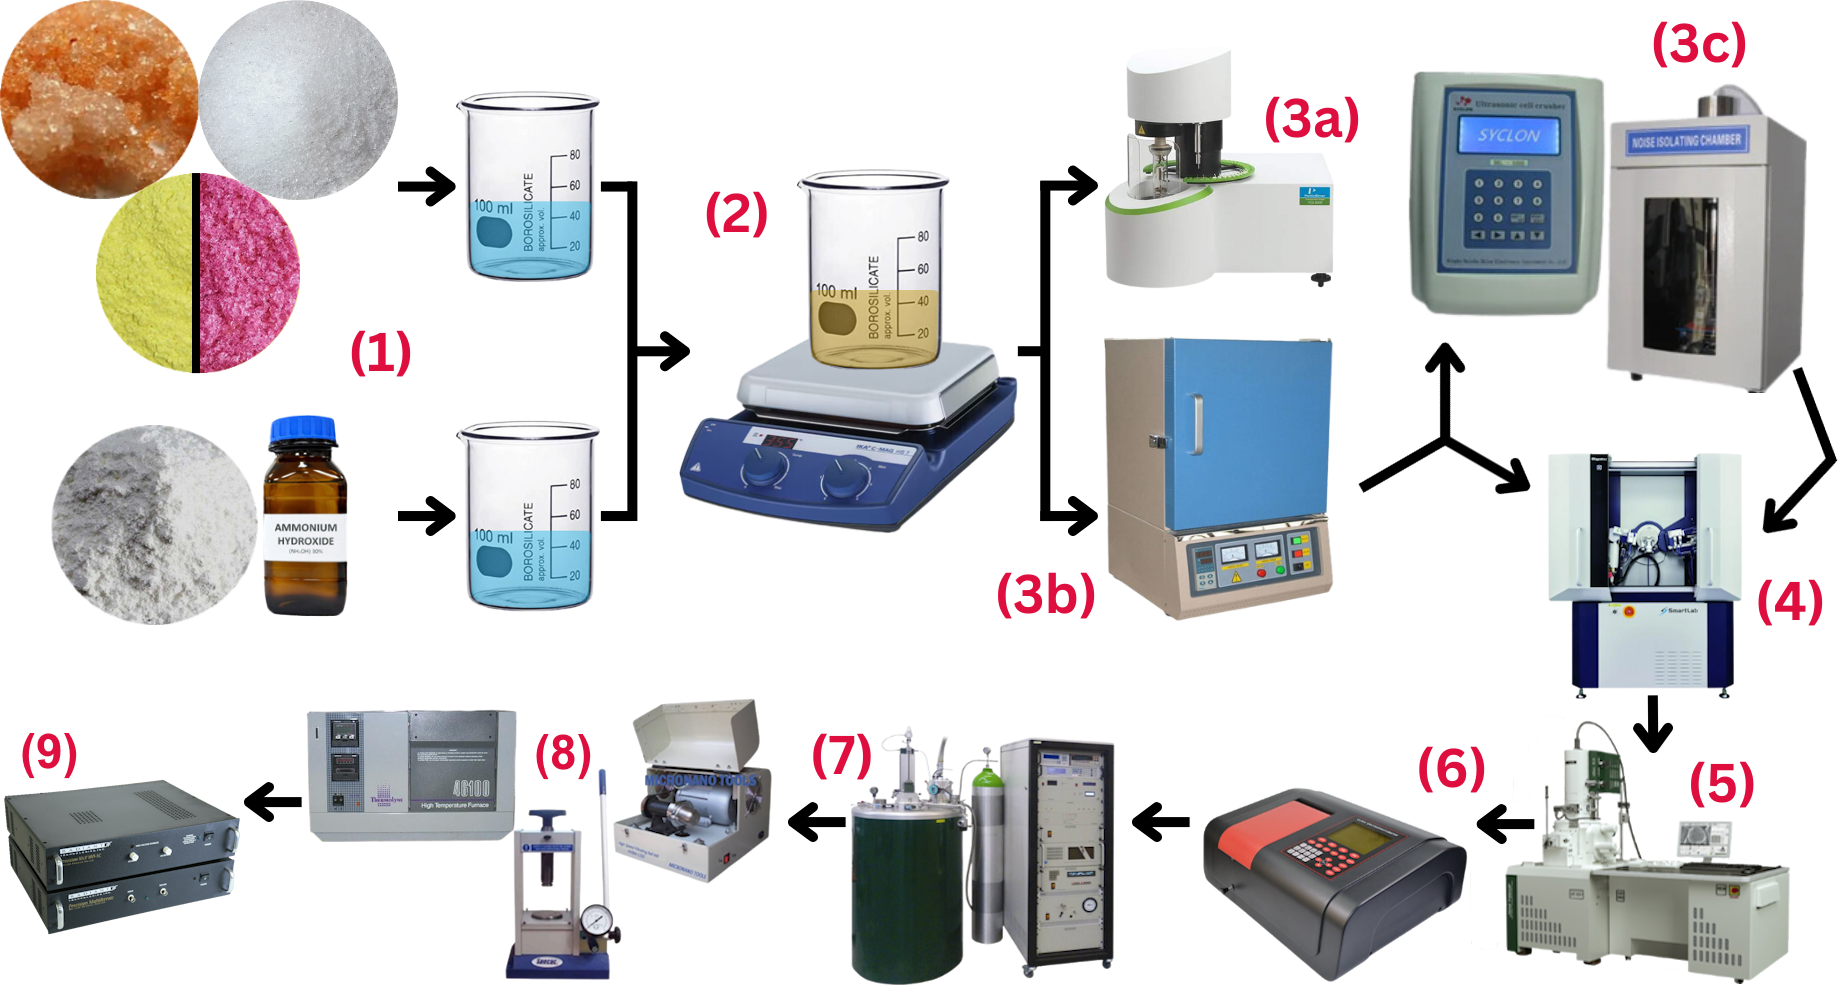
\includegraphics[width=0.75\textwidth]{fig/2.png}
    \caption{Diagrama de flujo del proceso de síntesis y caracterización seguido.}
    \label{fig:diagflujosint}
\end{figure}
\section{Síntesis}
En el caso del \neod{} se utilizaron los reactivos \ce{Fe(NO3)3} (Nitrato de Hierro (III)), \ce{Nd(NO3)3} (Nitrato de Neodimio (III)), \ce{C6H8O7} (ácido cítrico) y \ce{C10H16N2O8} (EDTA), además de \ce{NH4OH} (Hidróxido de Amonio), que se utiliza para disolver el EDTA en agua, además de neutralizar el pH de la mezcla. Mediante una relación estequiométrica, se obtuvieron las cantidades que se muestran en la Tabla \ref{tab:sintesisneod} por cada gramo de \ce{NdFeO3} sintetizado:
    \begin{table}[H]
        \centering
        \begin{tabular}{|c|c|}
        \hline
        Compuesto&Masa\\
        \hline
        \ce{Fe(NO3)3}&1.628g\\
        \ce{Nd(NO3)3}&1.7665g\\
        \ce{C6H8O7}&0.774g\\
        \ce{C10H16N2O8}&1.1775g\\
        \hline
    \end{tabular}
    \caption{Cantidad de cada compuesto necesaria para sintetizar 1g de \neod{}.}
    \label{tab:sintesisneod}
    \end{table}
    Por otro lado, para la síntesis del \sama{} se utilizaron los mismos reactivos a excepción del \ce{Nd(NO3)3}, el cuál fue sustituido por \ce{Sm(NO3)3} (Nitrato de Samario (III)). La relación estequiométrica por cada gramo es la que se muestra en la Tabla \ref{tab:sintesissama}:
    \begin{table}[H]
        \centering
        \begin{tabular}{|c|c|}
        \hline
        Compuesto&Masa\\
        \hline
        \ce{Fe(NO3)3}&1.5875g\\
        \ce{Sm(NO3)3}&1.7465g\\
        \ce{C6H8O7}&0.755g\\
        \ce{C10H16N2O8}&1.1485g\\
        \hline
    \end{tabular}
    \caption{Cantidad de cada compuesto necesaria para sintetizar 1g de \sama{}.}
    \label{tab:sintesissama}
    \end{table}
    En cada caso, los reactivos se mezclaron en dos vasos de precipitados con 20ml de agua destilada cada uno, el EDTA y el hidróxido de amonio en un vaso y el resto de los compuestos en otro, como se observa en la Figura \ref{fig:diagflujosint}.1, se calentó el vaso que contenía EDTA a alrededor de 60\gradoC{} mientras este se disolvía y posteriormente se añadió el contenido del otro vaso de precipitados. Posteriormente se comprobó que se tuviera un pH neutro y se subió la temperatura gradualmente hasta que la mezcla alcanzó alrededor de 80\gradoC{}, lo cual se ilustra en la Figura \ref{fig:diagflujosint}.2, esto con el fin de que se combustionara. Finalmente, el producto de esta combustión se molió haciendo uso de un mortero. 
    
    Una muestra tomada hasta este paso de la síntesis por cada tierra rara se separó para realizar un análisis termogravimétrico, mostrado en la Figura \ref{fig:diagflujosint}.3a, del cual se hablará en una sección posterior.

    El resto de muestras se calcinó por 12 horas, indicado en la Figura \ref{fig:diagflujosint}.3b haciendo uso de un horno BR-12N-3 de la marca Brother Furnace, con una rampa de calentamiento de 10\gradoC{}/min al subir la temperatura y 720 minutos constante en la temperatura objetivo. En cada muestra se utilizó una temperatura de calcinación distinta, ésta fue variada con intervalos de 100\gradoC{} entre cada muestra, empezando en 500\gradoC{} (600\gradoC{} en el caso del \sama{}) y terminando en 1000\gradoC{}.
\subsection{Sonicación}
    Además de esto, se sintetizaron dos muestras adicionales de \neod{} calcinada a 600\gradoC{} y \sama{} calcinada a 700\gradoC{}, a estas se les sometió a un proceso de sonicación a 292W, una por 2h y otra por 4h, lo cual se muestra en la Figura \ref{fig:diagflujosint}.3c.

    Esta técnica funciona a través de un generador electrónico que transforma una entrada de corriente alterna a una señal de 20kHz, la cual controla un convertidor piezoeléctrico para generar vibraciones mecánicas de alta frecuencia, las cuales son transmitidas a una punta ultrasónica la cual se sumerge en una solución que consiste en la muestra a sonicar y agua destilada. Las vibraciones de la punta generan burbujas microscópicas, en un fenómeno conocido como cavitación. Éstas, al colapsar, liberan una gran cantidad de energía, la cual es suficiente para romper las partículas en suspensión \cite{sonicaciondef}.

    La potencia de sonicación está limitada por la punta utilizada, en este caso el fabricante indica que el máximo para la punta utilizada es el 45\% de la potencia máxima del equipo, lo que equivale a 292W.
\section{Caracterización}

\subsection{Análisis Termogravimétrico (TGA)}
Esta técnica de caracterización, cuyo equipo se observa en la Figura \ref{fig:diagflujosint}.3a, y un diagrama de su estructura en la Figura \ref{fig:diagTGA}, consiste en pesar continuamente una muestra mientras se calienta, la cuál se encuentra en una atmósfera de gas inerte. Muchos sólidos experimentan reacciones que producen subproductos gaseosos, estos subproductos gaseosos se eliminan y se registran los cambios en la masa restante de la muestra. Mediante éste es posible encontrar la temperatura a la que ocurren distintas transformaciones en la sustancia, sean estas reacciones químicas, o cambios físicos, como la cristalización.
\begin{figure}[H]
    \centering
    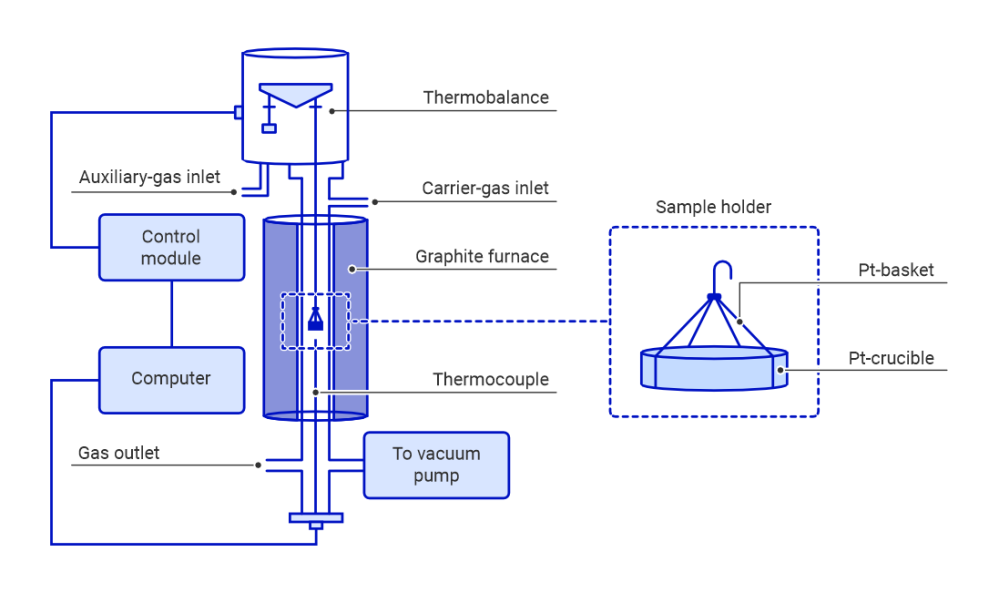
\includegraphics[width=0.7\textwidth]{fig/tgadiag.png}
    \caption{Diagrama de las partes que componen al equipo necesario para realizar un TGA. Adaptado de \cite{TGADIAG}.}
    \label{fig:diagTGA}
\end{figure}
Los procesos que se observan mediante esta técnica pueden ser endo o exotérmicos, debido a que tienen un efecto en el cambio de temperatura del material, sin embargo, dado que esta técnica no mide directamente la energía térmica de la muestra, no es posible diferenciar entre estos procesos sólo con los datos obtenidos mediante esta técnica \cite{TGA}.

Sin embargo, es posible inferir información sobre la posible temperatura a la que ocurre la cristalización al comparar los datos obtenidos con la temperatura de los cambios que se espera ocurran en la muestra. En este caso, se espera que haya una combustión de la fase orgánica de la muestra entre los 100 y 200\gradoC{}, mientras que la fase metálica es estable hasta temperaturas mucho más altas que las máximas alcanzadas por el equipo ($\approx1000$\gradoC{}), por lo que es posible asociar un proceso que ocurra a una temperatura mayor a 200\gradoC{} a la cristalización.
\subsection{Difracción de Rayos X (DRX)}
Esta técnica, cuyo equipo se puede observar en la Figura \ref{fig:diagflujosint}.4 se basa en la interferencia constructiva que ocurre al irradiar una muestra cristalina con un haz de rayos X monocromados en ángulos que dependen de las fases que contenga la muestra. Funciona a través de un tubo de rayos catódicos que bombardea con electrones a un objetivo, los cuales, al tener la energía suficiente, desplazarán los electrones más internos de los átomos del objetivo a niveles energéticos más altos, los cuales a su vez, al regresar al estado de menor energía liberan rayos X de una longitud de onda característica que depende el material objetivo utilizado, los cuales irradian la muestra que se quiere medir en un arreglo óptico como el que se ilustra en la Figura \ref{fig:diagDRX}, lo cual brinda información sobre las fases contenidas en la muestra, como se explicará en las siguientes secciones \cite{dutrowxrd}.
\begin{figure}[H]
    \centering
    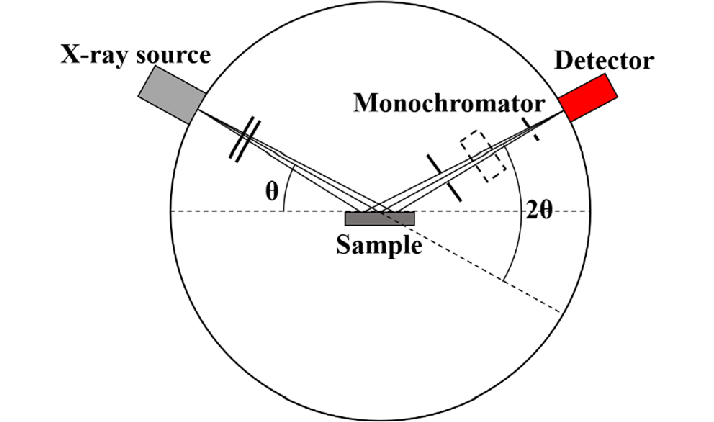
\includegraphics[width=0.6\textwidth]{fig/DRXdiag.png}
    \caption{Arreglo óptico utilizado para la obtención de espectros de difracción de rayos X. Adaptado de \cite{Jung2023}}
    \label{fig:diagDRX}
\end{figure}
\subsubsection{Estructura Cristalina}
Los átomos y moléculas que conforman la mayoría de sólidos, como el cuarzo, la sal, los metales o los óxidos, se encuentran en un arreglo periódico regular, ésto se conoce como cristalinidad, y a la estructura periódica como estructura cristalina.

Pensando en cada átomo pertenecientes a un cristal como un punto, podemos expresar un cristal en 3 dimensiones como el conjunto de puntos que cumplen:
$$\pmb{R}=\sum_{i=1}^{3} n_i\pmb{a_i}$$
Donde $\pmb{a_i}$ son vectores no colineales que representan cada dirección del cristal, cuyo tamaño es la separación entre átomos en esa dirección, además, $0\leq n_i<N_i$ es un número entero, donde $N_i$ es el tamaño máximo del cristal en esa dirección \cite{Ashcroft1976}.

La estructura que forma esta construcción, incluyendo los ángulos entre cada vector $\pmb{a_i}$, se conoce como red de Bravais. Existen sólo 14 posibles redes, como se puede ver en la Figura \ref{bravais} las cuáles pueden definirse a través de su celda unitaria, que representa la unidad mínima del cristal que, al repetirse periódicamente en todas direcciones, genera el cristal entero.
\begin{figure}[H]
    \centering
    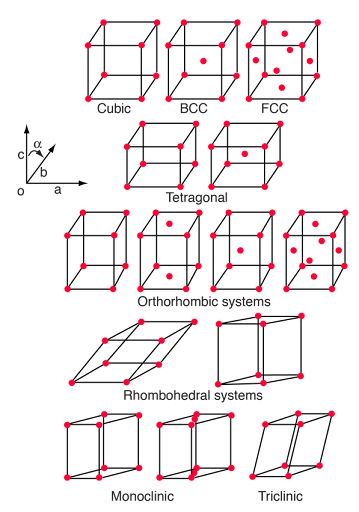
\includegraphics[width=0.75\textwidth]{fig/bravais.png}
    \caption{Redes de Bravais. Adaptado de \cite{ScienceFacts2024}.}
    \label{bravais}
\end{figure}
Es posible expresar la orientación de cualquier plano que corte la estructura cristalina a través de los índices de Miller, éstos se obtienen a partir de las distancias entre el origen y los puntos en los que el plano intersecta a los ejes, expresado como fracciones de la distancia entre átomos en ese eje. Si se tomaran directamente estas distancias, no se podría tratar directamente con planos perpendiculares a los generados por los ejes, debido a que la intersección entre estos ocurre en el $\infty$, por esta razón, los índices de Miller se definen a través del recíproco de estas distancias, tomando 0 como recíproco de $\infty$, dando como resultado 3 números $h$, $k$, $l$, que se expresan como $(hkl)$, como se observa en la Figura \ref{millerdiag}a, si alguno fuese negativo, se escribe con una barra encima, $\left(\bar{h}kl\right)$. Finalmente, los 3 números obtenidos se multiplican por una constante para obtener el conjunto de enteros más pequeños generable con la menor cantidad de números negativos para ese trío de números, es decir, $(102)$ es correcto, pero $(204)$ o $\left(\frac{1}{2}01\right)$ no lo es \cite{Cullity2014}, un ejemplo de esta asignación puede verse en la Figura \ref{millerdiag}b.
\begin{figure}[H]
    \centering
    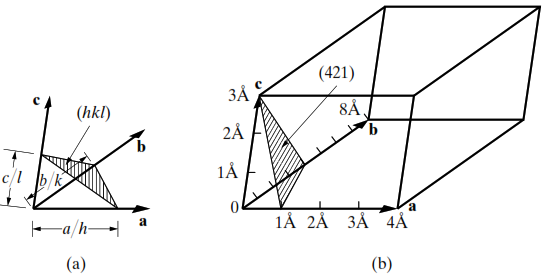
\includegraphics[width=0.7\textwidth]{fig/miller.png}
    \caption{Asignación de índices de Miller. Tomado de \cite{Cullity2014}.}
    \label{millerdiag}
\end{figure}
\paragraph{Ley de Bragg}

\subsubsection{Modelado de Picos de Difracción}

\paragraph{Justificación Teórica}

\paragraph{Factores de Bondad}

\subsubsection{Fórmula de Scherrer}

\subsection{Microscopía Electrónica de Barrido (SEM)}

\subsubsection{Conceptos para el Análisis Estadístico}

\subsubsection{Morfología}

\subsubsection{EDS}

\subsection{Espectroscopía UV-Vis}

\subsubsection{Método Tauc}

\subsection{Magnetometría}

\subsubsection{Dispositivo Superconductor de Interferencia Cuántica (SQUID)}

\paragraph{\textit{Zero Field Cooling} y \textit{Field Cooling}}

\paragraph{Mediciones Magnéticas Realizadas}

\end{document}